% !TEX TS-program = pdflatex
% !TEX encoding = UTF-8 Unicode

% This is a simple template for a LaTeX document using the "article" class.
% See "book", "report", "letter" for other types of document.

\documentclass[11pt]{article} % use larger type; default would be 10pt

\usepackage[utf8]{inputenc} % set input encoding (not needed with XeLaTeX)
\usepackage[spanish]{babel}

%%% Examples of Article customizations
% These packages are optional, depending whether you want the features they provide.
% See the LaTeX Companion or other references for full information.

%%% PAGE DIMENSIONS
\usepackage{geometry} % to change the page dimensions
\geometry{a4paper} % or letterpaper (US) or a5paper or....
% \geometry{margin=2in} % for example, change the margins to 2 inches all round
% \geometry{landscape} % set up the page for landscape
%   read geometry.pdf for detailed page layout information

\usepackage{graphicx} % support the \includegraphics command and options
\usepackage[outdir=./]{epstopdf}
% \usepackage[parfill]{parskip} % Activate to begin paragraphs with an empty line rather than an indent
\usepackage{listings}

%%% PACKAGES
\usepackage{booktabs} % for much better looking tables
\usepackage{array} % for better arrays (eg matrices) in maths
\usepackage{paralist} % very flexible & customisable lists (eg. enumerate/itemize, etc.)
\usepackage{verbatim} % adds environment for commenting out blocks of text & for better verbatim
%\usepackage{subfig} % make it possible to include more than one captioned figure/table in a single float
\usepackage{subcaption}
\usepackage{url}
\usepackage{diagbox}
\usepackage{amsmath}
\usepackage{pdfpages}
% These packages are all incorporated in the memoir class to one degree or another...

%%% HEADERS & FOOTERS
\usepackage{fancyhdr} % This should be set AFTER setting up the page geometry
\pagestyle{fancy} % options: empty , plain , fancy
\renewcommand{\headrulewidth}{0pt} % customise the layout...
\lhead{}\chead{}\rhead{}
\lfoot{}\cfoot{\thepage}\rfoot{}

%%% SECTION TITLE APPEARANCE
\usepackage{sectsty}
\allsectionsfont{\sffamily\mdseries\upshape} % (See the fntguide.pdf for font help)
% (This matches ConTeXt defaults)

%%% ToC (table of contents) APPEARANCE
\usepackage[nottoc,notlof,notlot]{tocbibind} % Put the bibliography in the ToC
\usepackage[titles,subfigure]{tocloft} % Alter the style of the Table of Contents
\renewcommand{\cftsecfont}{\rmfamily\mdseries\upshape}
\renewcommand{\cftsecpagefont}{\rmfamily\mdseries\upshape} % No bold!

%%% END Article customizations

%%% The "real" document content comes below...

\title{CLP Lab 7 Report}
\author{Albert Aparicio Isarn\\
	\url{albert.aparicio.isarn@alu-etsetb.upc.edu}
	\and
	Héctor Esteban Cabezos\\
	\url{hect.esteban@gmail.com}}
\date{} % Activate to display a given date or no date (if empty),
         % otherwise the current date is printed

\begin{document}

	% ---- MATLAB Code definitions ----- %
	\definecolor{mygreen}{rgb}{0,0.6,0}
	\definecolor{mygray}{rgb}{0.5,0.5,0.5}
	\definecolor{mymauve}{rgb}{0.58,0,0.82}

	\lstset{ %
		%backgroundcolor=\color{white},   % choose the background color; you must add \usepackage{color} or \usepackage{xcolor}
		basicstyle=\ttfamily\footnotesize,        % the size of the fonts that are used for the code
		breakatwhitespace=false,         % sets if automatic breaks should only happen at whitespace
		breaklines=true,                 % sets automatic line breaking
		captionpos=b,                    % sets the caption-position to bottom
		commentstyle=\color{mygreen},    % comment style
		deletekeywords={...},            % if you want to delete keywords from the given language
		escapeinside={\%*}{*)},          % if you want to add LaTeX within your code
		extendedchars=true,              % lets you use non-ASCII characters; for 8-bits encodings only, does not work with UTF-8
		%frame=single,	                   % adds a frame around the code
		keepspaces=true,                 % keeps spaces in text, useful for keeping indentation of code (possibly needs columns=flexible)
		keywordstyle=\color{blue},       % keyword style
		language=Matlab,                 % the language of the code
		otherkeywords={*,...},            % if you want to add more keywords to the set
		%numbers=left,                    % where to put the line-numbers; possible values are (none, left, right)
		%numbersep=5pt,                   % how far the line-numbers are from the code
		%numberstyle=\tiny\color{mygray}, % the style that is used for the line-numbers
		rulecolor=\color{black},         % if not set, the frame-color may be changed on line-breaks within not-black text (e.g. comments (green here))
		showspaces=false,                % show spaces everywhere adding particular underscores; it overrides 'showstringspaces'
		showstringspaces=false,          % underline spaces within strings only
		showtabs=false,                  % show tabs within strings adding particular underscores
		stepnumber=2,                    % the step between two line-numbers. If it's 1, each line will be numbered
		stringstyle=\color{mymauve},     % string literal style
		tabsize=2,	                   % sets default tabsize to 2 spaces
		title=\lstname                   % show the filename of files included with \lstinputlisting; also try caption instead of title
	}

\maketitle

\section{Programación de método de clasificación}

El script \textbf{\texttt{main\_2\_1}} contiene el código del ejercicio 1. En
la sección \ref{src:main:21} se puede ver su código fuente.

La sección 2 de este ejercicio corresponde a la función
\textbf{\texttt{CLP\_Kmeans}}, cuyo código fuente se muestra en la sección
\ref{src:fun:kmeans}.

A continuación se muestran los resultados de este ejercicio. En la figura
\ref{fig:21:clusters} se muestra la base de datos creada
por \textbf{\texttt{CLP\_Generate}} (código fuente en la sección
\ref{src:clp:generate}) y el resultado de la clasificación con 4, 9 y 10
\emph{clusters}.

% TODO Posar correctament les captions i labels
\begin{figure}[h]
	\centering
	\begin{subfigure}[b]{0.435\textwidth}
		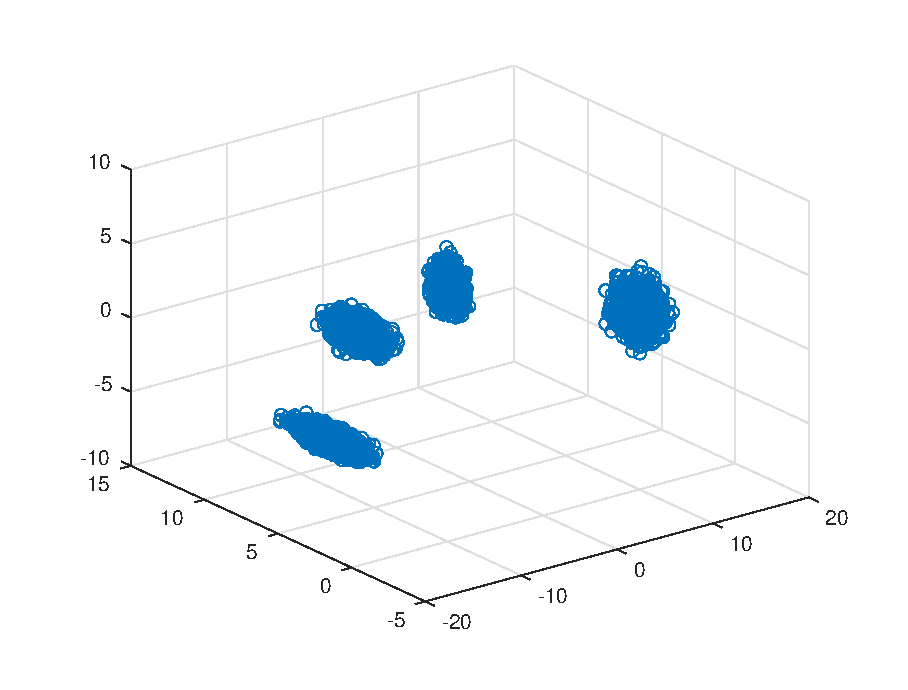
\includegraphics[width=\textwidth]{../src/fig/21_database.eps}
		\caption[]{\small $P_{min} = 0.75$}
		\label{fig:db:075}
	\end{subfigure}
        \quad
        \begin{subfigure}[b]{0.435\textwidth}
                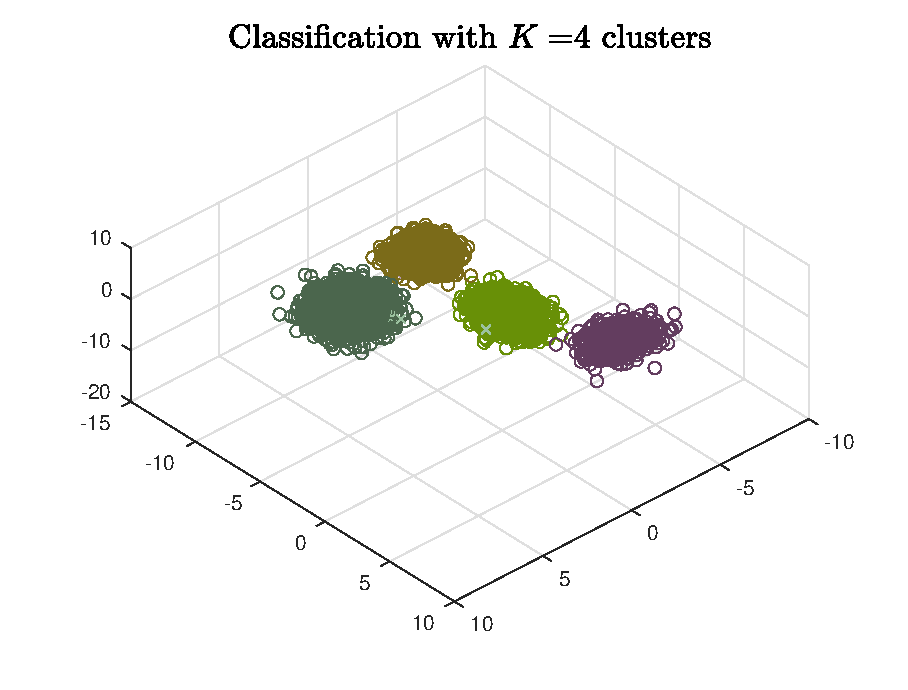
\includegraphics[width=\textwidth]{../src/fig/21_4_clusters.eps}
                \caption[]{\small $P_{min} = 0.85$}
                \label{fig:db:085}
        \end{subfigure}
        \vskip\baselineskip
        \begin{subfigure}[b]{0.435\textwidth}
                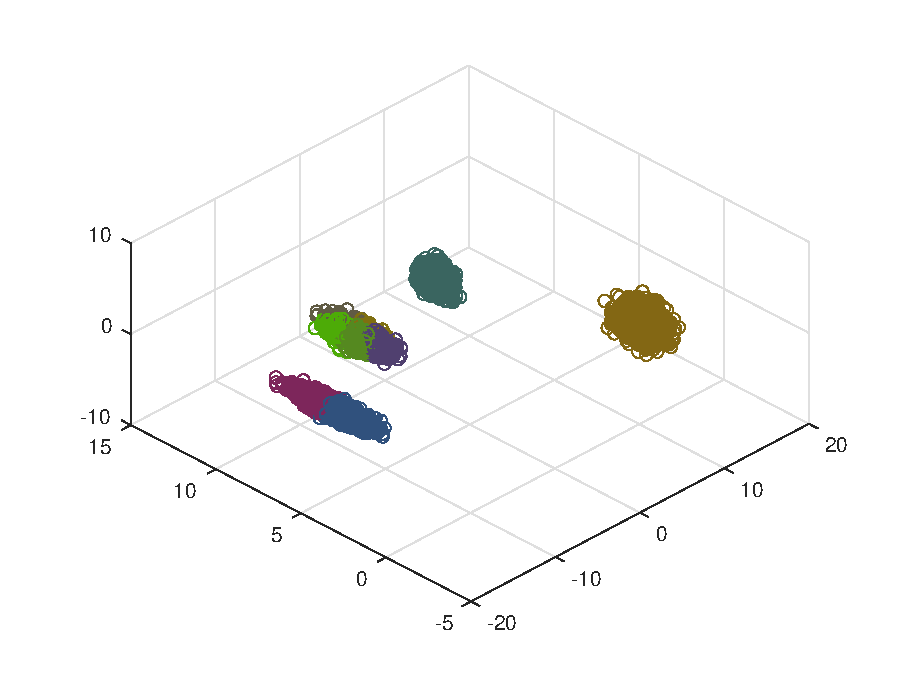
\includegraphics[width=\textwidth]{../src/fig/21_9_clusters.eps}
                \caption[]{\small $P_{min} = 1$}
                \label{fig:db:100}
        \end{subfigure}
        \quad
        \begin{subfigure}[b]{0.435\textwidth}
                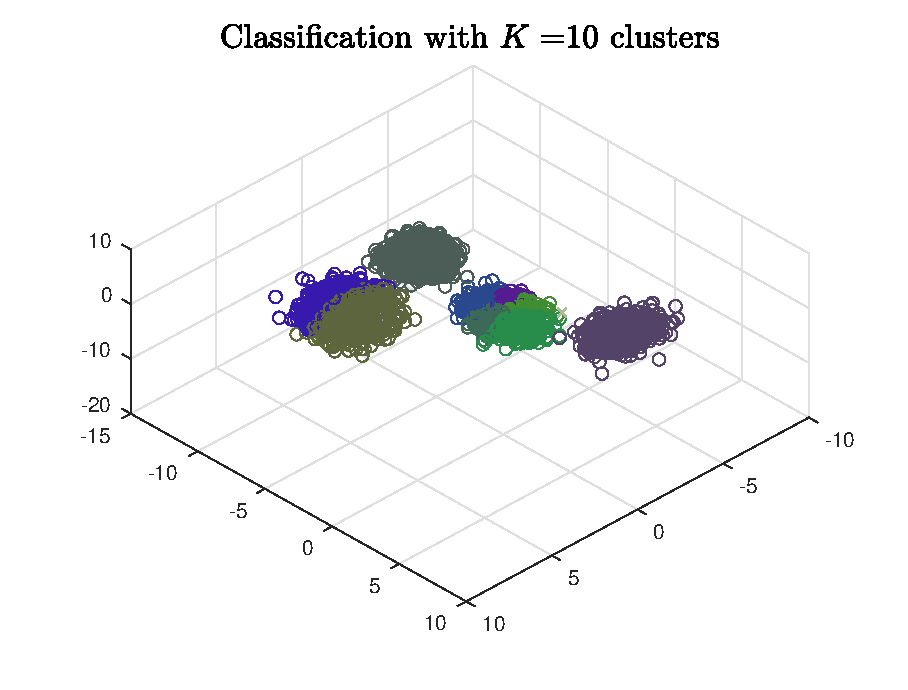
\includegraphics[width=\textwidth]{../src/fig/21_10_clusters.eps}
                \caption[]{\small $P_{min} = 0.85$}
                \label{fig:db:085}
        \end{subfigure}
	\caption{Imagenes resultantes de las labels con varios valores de $P_{min}$}
	\label{fig:db}
\end{figure}

\section{Cuantificación de imágenes}

More text.

\section{Identificación de clústeres en una base de datos propia}

\section{Código fuente}
\label{sec:src_code}

A continuación se encuentra el código fuente generado para la resolución de
este laboratorio

\subsection{\texttt{main\_2\_1}}
\label{src:main:21}

\lstinputlisting{../src/main_2_1.m}

% TODO Codi font CLP_Generate

\subsection{\texttt{CLP\_Kmeans}}
\label{src:fun:kmeans}

\lstinputlisting{../src/CLP_Kmeans.m}

\end{document}
